\chapter{选学：CUDA 激光雷达加速}
\begin{notebox}
\textbf{目标}\quad 保留 CPU 基线，逐束验证 GPU 结果，并分清计算、传输和完整消息成本。\\
\textbf{先修}\quad 第 05 章、C++ 数组；不要求为前面章节安装 CUDA。
\end{notebox}
\section{先建立可复现的工具链}
默认 CPU 构建不查找 CUDA。本机使用 RTX 5060、驱动 595.91.07、GCC 15.2 和 CUDA 13.2.1。
主机原先缺少 nvcc；脚本将官方组件按锁定 SHA-256 下载到 tmp，保留许可证，不修改驱动。
13.0.2 与本机 glibc 2.43 的头文件冲突，故选用已实测的 nvcc 13.2.78。
\begin{lstlisting}[language=bash]
# Repository root; optional Linux x86_64 toolchain
python3 scripts/setup_cuda_local.py
source /opt/ros/lyrical/setup.bash
cd ros2_ws
colcon build --symlink-install --cmake-args \
  -DCMAKE_BUILD_TYPE=RelWithDebInfo \
  -DPython3_EXECUTABLE=/usr/bin/python3
colcon build --packages-select motion2d --symlink-install \
  --cmake-args -DMOTION2D_ENABLE_CUDA=ON \
  -DCMAKE_CUDA_COMPILER="$PWD/../tmp/cuda-13.2.1/toolkit/bin/nvcc" \
  -DCMAKE_CUDA_HOST_COMPILER=/usr/bin/g++ \
  -DCMAKE_CUDA_ARCHITECTURES=120
source install/setup.bash
ros2 run motion2d lidar_cuda_benchmark > ../tmp/ch20_cuda.csv
\end{lstlisting}
120 是本机 GPU 的计算能力，不适用于所有显卡。现代 CMake 可使用 native 探测本机；
跨机器运行时需按目标选择架构。
禁用时将上述 CUDA 开关显式设为 OFF；CMake 会记住旧设置，只删掉命令中的 ON 不能将它关闭。

\section{同一接口，不改变测量含义}
CudaLidar 构造时接收静态世界及最大束数，scan 接收位姿和相同 LidarConfig，返回相同 float 数组。
扫描仍是圆心处的瞬时均匀扫描；完整一周用 $2\pi/N$，部分视场包含两端。
近于最小量程为 NaN，超出最大量程为 $+\infty$，不能把二者都解释为自由空间。

设备几何使用 double，输出才转为 float；本实验关闭 FMA 融合，没有 fast-math。
这些选择便于与 CPU 对照，但不是最高性能方案。
相同误差 $e_i$ 在两个无噪声输出上分别调用 perturbRange；不能仅凭“两个独立生成器种子相同”
就认定样本相同，因为不同后端的生成顺序或特殊值跳过方式可能不同。

\clearpage
\section{一束一个线程}
第 $i$ 束仍计算
\begin{equation}
 \theta_i=\psi+\theta_{\min}+i\Delta\theta,\qquad
 d_i=\min\{d_{i,\rm circles},d_{i,\rm edges},d_{i,\rm walls}\}.
\end{equation}
一束对应一个线程；线程内部遍历所有圆和边，顺序求最小命中。
本章没有再做障碍物并行归约，也没有 BVH；先保持与 CPU 公式逐行可比。
B 束、C 个圆、E 条边的总工作量仍为 $O(B(C+E))$，并行只改变执行安排。
\lstinputlisting[language=C++,linerange={cuda_rays_begin-cuda_rays_end},includerangemarker=false]{../ros2_ws/src/motion2d/src/sim/lidar_cuda.cu}

每块 128 个线程，总块数为 $\lceil B/128\rceil$；末块多出的线程通过边界判断返回。
几何打包成一个连续的结构分量数组：圆的 cx、cy、r，然后是边的 ax、ay、bx、by。
外框也作为四条边加入；所有线程复用这些静态数据。
相邻线程读取相同障碍物参数，有利于缓存复用，但不能仅凭采用 SoA 就声称已经更快。

\paragraph{内存与生命周期}
构造时分配设备几何、输出数组和计时事件，上传一次；后续扫描重复使用。
位姿和角度等少量标量作为内核参数传入，输出仍须回传 CPU，供噪声和 ROS 消息使用。
此版本使用默认流、同步返回，暂不引入多流、双缓冲和跨帧异步调度。
CudaLidar 是一个小类，其内部 CUDA 资源只存在于可选实现中，CPU 头文件不依赖 CUDA Runtime。

\paragraph{先检查正确性}
GPU 测试覆盖 40 个自由随机位姿、圆相切、共线边、部分视场、NaN 与无回波，
逐束分别比较特殊值类别和有限距离，容差为 $2\times10^{-5}$ m。
再施加同一批噪声样本并重复检查。启用 CUDA 却没有可用 GPU 时测试应失败，
不能静默切到 CPU 后仍报告“GPU 验收通过”。

\clearpage
\section{完整扫描收益取决于规模}
\begin{lstlisting}[language=bash]
# Copy benchmark CSV to textbook/data only when recording a new run.
python3 scripts/plot_ch20_cuda.py
\end{lstlisting}
每组预热 20 次，再运行 60 次，分别记录 P50/P95；CPU 与 GPU 使用相同位姿和几何。
0/16/128/512 个障碍物、90/720/4096/16384 束共 16 组，圆与四边形各占一半，
外框另计四条边。计时场景为独立合成夹具，不把随机生成器的连通性筛选时间计入扫描。

\begin{figure}[!ht]
\centering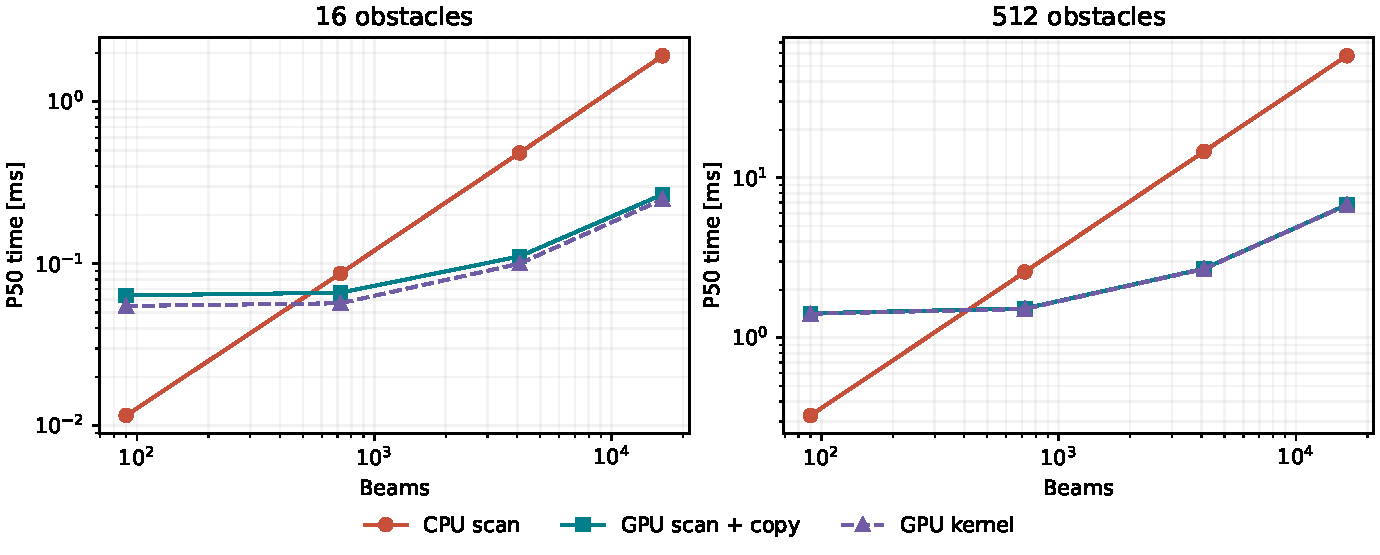
\includegraphics[width=\linewidth]{figures/ch20_cuda.pdf}
\caption{RTX 5060 主机实测，两个坐标轴都用对数。
驻留 GPU 扫描包含内核启动、同步和结果回传；虚线只表示内核，不能替代整条曲线。}
\end{figure}

\begin{center}\small
\begin{tabular}{rrrrr}\toprule
障碍/束 & CPU/ms & 内核/ms & 驻留扫描/ms & CPU/扫描\\\midrule
16/90 & 0.0116 & 0.0549 & 0.0638 & 0.18\\
16/720 & 0.0873 & 0.0571 & 0.0663 & 1.32\\
16/16384 & 1.923 & 0.250 & 0.267 & 7.19\\
512/90 & 0.327 & 1.413 & 1.422 & 0.23\\
512/16384 & 57.913 & 6.766 & 6.784 & 8.54\\\bottomrule
\end{tabular}
\end{center}
表中均为预热后的 P50。少量束时 GPU 明显更慢：并行度不足、启动固定成本和 double 算术代价
可能超过并行收益。720 束、16 障碍只有约 1.32 倍驻留扫描收益，不能写成数量级加速。

一次 setup 包括主机打包、分配、上传和事件创建；首组约 61 ms，还可能包含上下文初始化。
之后的 setup 约 0.029--0.110 ms；单独上传约 0.002--0.012 ms，不应每帧重复支付。
回传约 0.005--0.013 ms，已包含在驻留扫描里；不能把三个独立分位数相加当作总时长分位数。
CUDA 事件测内核，墙钟测同步后的回传和整次扫描；只量异步 launch 的返回时间会严重低估成本。

本次 16 组输出的 float 距离最大差为 0，随机位姿与噪声检查也通过；
这不是所有场景位级一致的承诺，仍保留浮点容差及特殊值检查。
练习 ch20-1 补齐 ray-circle 根选择，并解释为什么增加障碍、但不增加束数，未必能让 GPU 获益。
完整 ROS 噪声、消息构建和发布成本仍需在节点中另测，不能由此表推断。
